\documentclass{article}
\usepackage{graphicx}
\usepackage{appendix}
\usepackage{csvsimple}
\title{Homework 1}
\author{Yuanyou Yao}
\begin{document}
\maketitle{}
\paragraph{Problem 1}
\subparagraph{MoM}~{}
\newline
Advantages:
\begin{enumerate}
\item Simple to generate Asymptotically normal (tends to normal when sample size n is large) 
\end{enumerate}
Disadvantages:
\begin{enumerate}
\item Inconsistent results (more than one estimator equation) 
\item Do not know how close the estimate is from parameter of interest
\end{enumerate}
\subparagraph{LS}~{}
\newline
Advantages:
\begin{enumerate}
\item LS can predict unknown data according to linear model beta is BLUE
\end{enumerate}
Disadvantages:
\begin{enumerate}
\item The method is a linear estimation. So it cannot be used in other distribution
\end{enumerate}
\subparagraph{MLE}~{}
\newline
Advantages:
\begin{enumerate}
\item Asymptotically unbiased, consistent, normally distributed, and efficient 
\end{enumerate}
Disadvantages: 
\begin{enumerate}
\item Can be highly biased for small samples
\item Sometimes, MLE has no closed-form
\end{enumerate}

The Univariate Gaussian Distribution:\[f(x)=\frac{1}{\sqrt{2\pi}\sigma}exp\frac{(x-\mu)^2}{2\sigma^2}\]

The  log-likelihood function of $f(x)$ is \[lnL(\mu,\sigma^2;x)=-\frac{n}{2}ln(2\pi \sigma^2)-\frac{1}{2\sigma^2}\sum_{i=1}^n(x_i-\mu)^2\]
and we let the partial differential equals 0, we get\[\mu=\frac{1}{n}\sum_{i=1}^nX_i=\bar{X}, \sigma^2=\frac{1}{n}\sum_{i=1}^n(X_I-\bar{X})^2\]
\paragraph{Problem2}
\subparagraph{a)}~{}
\newline
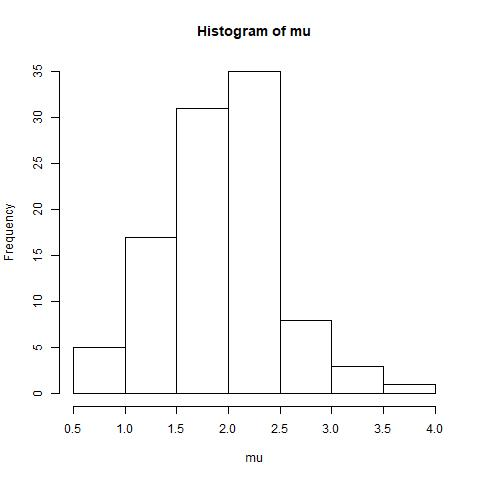
\includegraphics[height=6cm,width=7cm]{2amean.jpg}
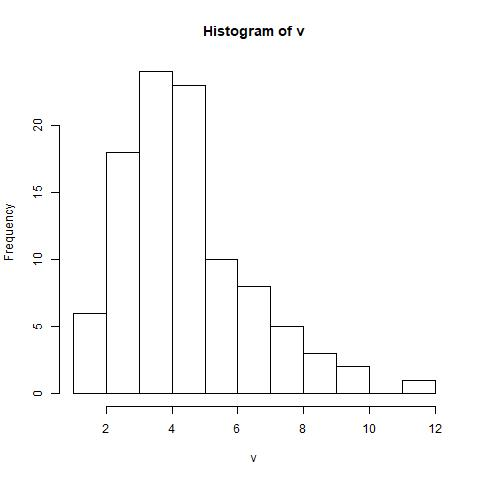
\includegraphics[height=6cm,width=7cm]{2avar.jpg}
\subparagraph{b)}~{}
\newline
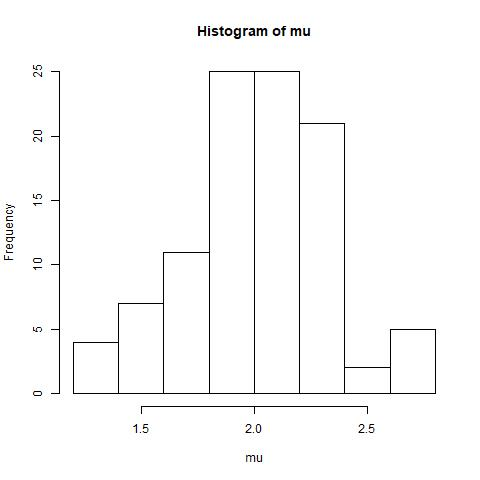
\includegraphics[height=6cm,width=7cm]{2bmean.jpg}
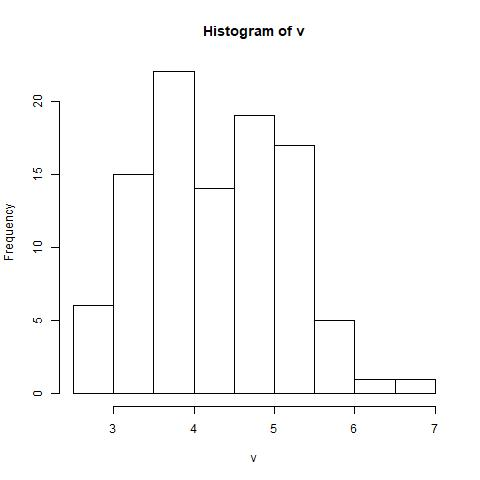
\includegraphics[height=6cm,width=7cm]{2bvar.jpg}
\subparagraph{c)}~{}
\newline
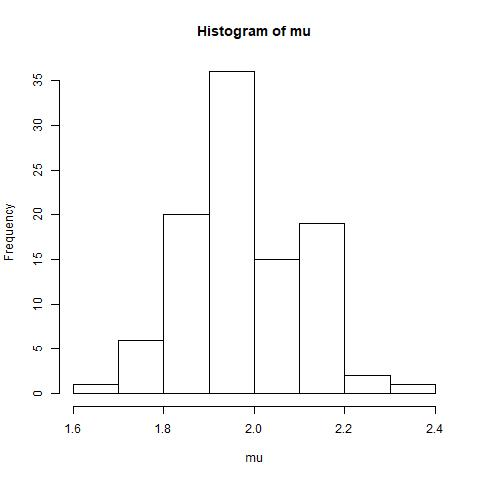
\includegraphics[height=6cm,width=7cm]{2cmean.jpg}
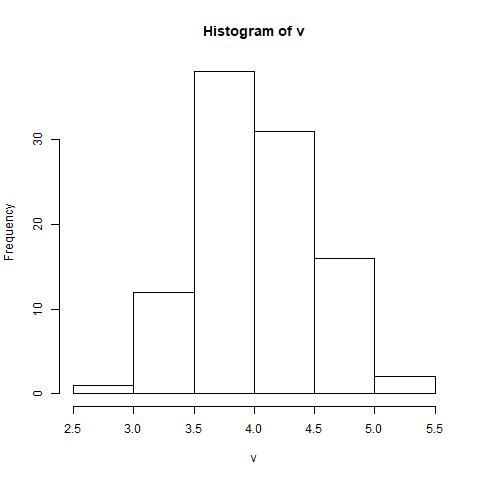
\includegraphics[height=6cm,width=7cm]{2cvar.jpg}
\subparagraph{d)}
As the observations become larger, the sample means and variances are closer to the population mean and variance.
\subparagraph{e)}~{}
\newline
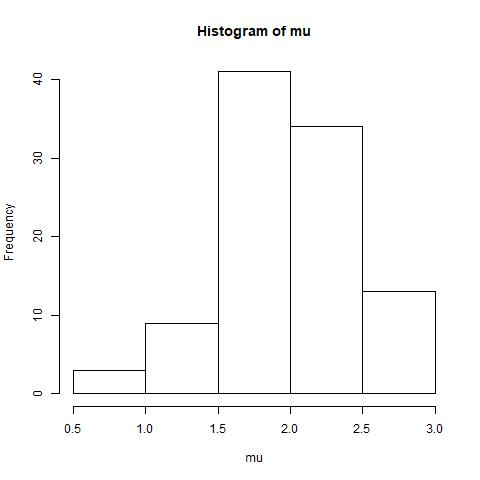
\includegraphics[height=6cm,width=7cm]{2emean.jpg}
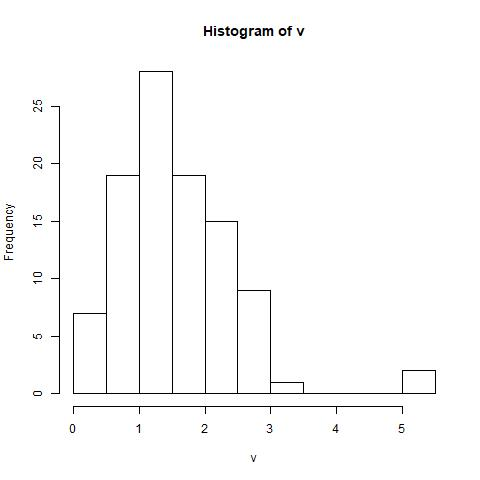
\includegraphics[height=6cm,width=7cm]{2evar.jpg}

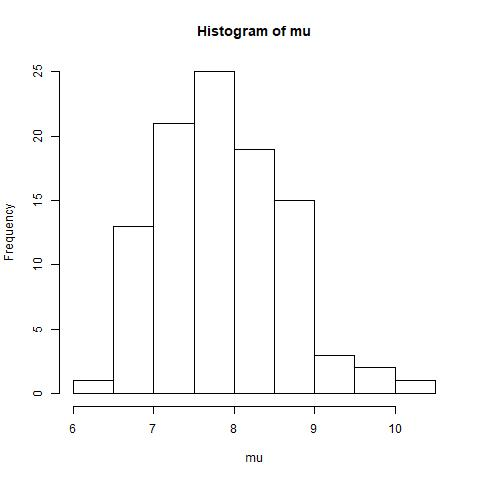
\includegraphics[height=6cm,width=7cm]{2emean40.jpg}
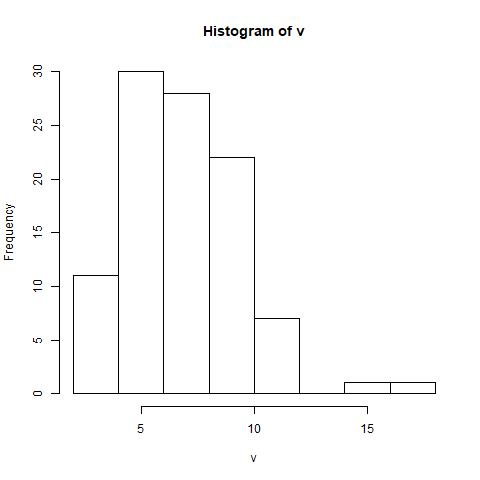
\includegraphics[height=6cm,width=7cm]{2evar40.jpg}

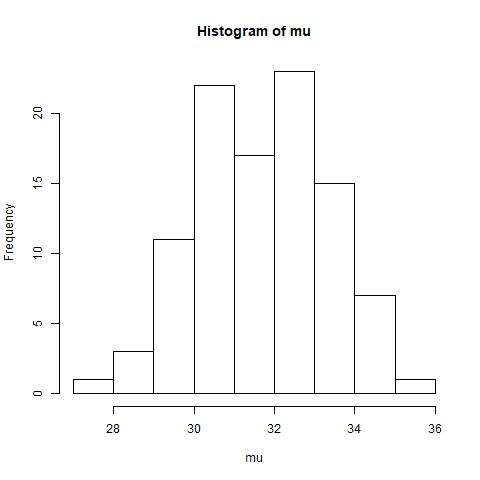
\includegraphics[height=6cm,width=7cm]{2emean160.jpg}
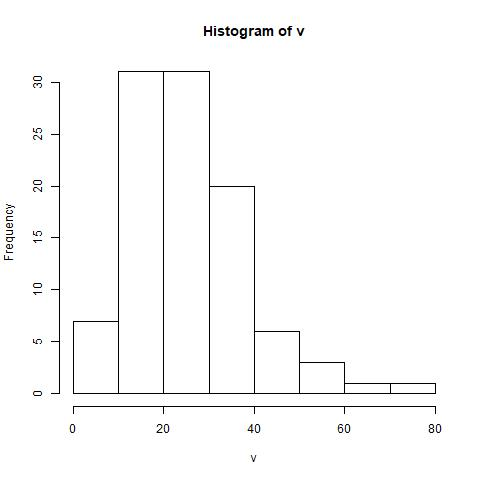
\includegraphics[height=6cm,width=7cm]{2evar160.jpg}
\subparagraph{f)}~{}

$E(\bar{Y})=\mu$,
$Var(\bar{Y})=\frac{\sigma^2}{n}$,
$E(S^2)=\sigma^2$

Comparing to the simulations:

a)$E(\bar{Y})=1.976704$,
$Var(\bar{Y})=0.2956425$,
$E(S^2)=4.430259$

b)$E(\bar{Y})=2.002061$,
$Var(\bar{Y})= 0.01577688$,
$E(S^2)=4.299138$

c)$E(\bar{Y})=1.977944$,
$Var(\bar{Y})=0.1005564$,
$E(S^2)=4.027052$

Conclusions:As the observations become larger, the statistics are closer to the theoretical value.

The difference between $Var(\bar{Y})$ and$Var(Y)$:$Var(Y)=\sigma^2$ while $Var(\bar{Y})=\frac{\sigma^2}{n}$. $var(Y)$ is the population variance while $var(\bar{Y})$is the sample variance.
\subparagraph{g)}~{}

$E(\bar{Y})=m\pi$,
$Var(\bar{Y})=\frac{m\pi(1-\pi)}{n}$,
$E(S^2)=m\pi(1-\pi)$

Comparing to the simulations:

n=10)$E(\bar{Y})=2.013$,
$Var(\bar{Y})=0.1791222$,
$E(S^2)=1.610556$

n=40)$E(\bar{Y})=1.98675$,
$Var(\bar{Y})= 0.03682393$,
$E(S^2)=1.663199$

n=160)$E(\bar{Y})=2.00225$,
$Var(\bar{Y})=0.008862468$,
$E(S^2)=1.625002$

Conclusions:As the observations become larger, the statistics are closer to the theoretical value.
\paragraph{Problem3}
\subparagraph{a)}~{}

$H_0:\mu=0$ vs $H_a:\mu!=0$, $\mu$ is the difference of mean of pretest and posttest
\subparagraph{b)}~{}
\newline
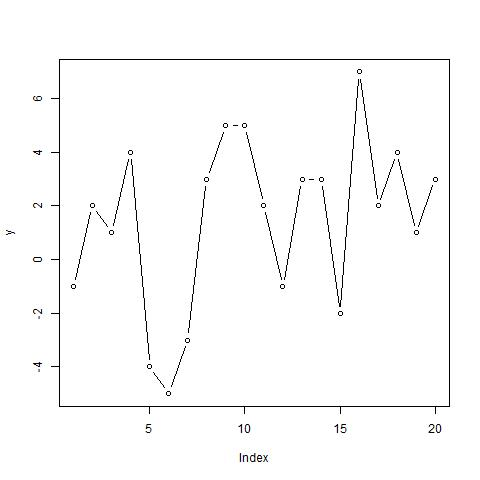
\includegraphics[height=6cm,width=7cm]{3b.jpg}

The graph shows that the difference of mean is near 0, so we have to use t test to determine the whether the scores are different or not.
\subparagraph{c)}
According to R, under 5\% chance of making mistakes, we can conclude that the training improves listening skills by true difference in means is not equal to 0.
\subparagraph{d)}
90 percent confidence interval:
 (-1.159166  , 4.059166)
\subparagraph{e)}~{}
We need to use the t statistics, that is,\[T=\frac{\bar{d}-\mu_0}{\frac{s_d}{\sqrt{n}}}=\frac{-1.45-0}{\frac{3.203206}{\sqrt{n}}}= −0.4526715\sqrt{n} \]
According to R, the minimum sample size n needed is 2.
\paragraph{Problem4}
\subparagraph{a)}~{}
\newline
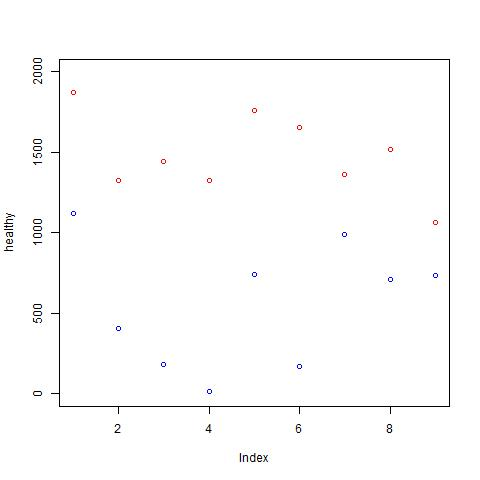
\includegraphics[height=6cm,width=7cm]{4a.jpg}

The red spots are from healthy buds and the blue spots are from virus-infected buds.

median(healthy) 1446;
median(infected) 577.5

mean(healthy) 1480;
mean(infected) 549.4286

sd(healthy) 248.9849;
sd(infected) 343.4586

Tentative Conclusions: The average of healthy stem volume is nearly three times as infected volume. Infected stem volume also has larger range from 16 cubic centimeters to 1121 cubic centimeters, which reflects as a larger standard deviation.
\subparagraph{b)}~{}

Hypothesis:\[H_0:\mu_1\leq \mu_2\] \[H_a:\mu_1> \mu_2\]

$\mu_1$ is the mean of healthy stem volume and $\mu_2$ is the mean of virus-infected volume.

then,we can find $\mu=\mu_1-\mu_2$, the hypothesis becomes:

\[H_0:\mu\leq 0\] \[H_a:\mu>0\]

We use the following formula:
\[\frac{(\mu_1-\mu_2)-0}{\sqrt{S^2(\frac{1}{n_1}+\frac{1}{n_2})}}\]

$S$ is a weighted average of the two sample variances, weighted by the d.f.’s
\[S=\frac{(n_1-1)S_1+(n_2-1)S_2}{n_1+n_2-2}\]

The result is $t=7.0063$ and the p-value is $p =6.446e-07$.

Since the p-value is much smaller than $\alpha=5\%$, It is safe to reject $H_0$ and say the mean stem volume of 2-year-old seedlings propagated from virus-infected buds is smaller than those propagated from healthy buds. 
\subparagraph{c)}~{}

Let $t_{n_1+n_2-2,\alpha/2}$ denote the t critical value such that 
\[CI=\bar{Y_1}-\bar{Y_2}\pm t_{n_1+n_2-2,\alpha/2}\times \sqrt{S^2(\frac{1}{n_1}+\frac{1}{n_2})}\]

So, a 95\% confidence interval for the difference of the mean stem volume of 2-year-old seedlings between the two groups is\[(654.3586,1206.7842)\]
\subparagraph{d)}The output of R running t.test: 

Two Sample t-test

data:  healthy and infected

t = 7.0063, df = 21, p-value = 6.446e-07

alternative hypothesis: true difference in means is not equal to 0

95 percent confidence interval:

  654.3586 1206.7842

sample estimates:

mean of x mean of y 

1480.0000  549.4286 

Interpretation: Since the p-value is much smaller than $\alpha=5\%$, It is safe to reject $H_0$ and say the mean stem volume of 2-year-old seedlings propagated from virus-infected buds is different from those propagated from healthy buds. 
\subparagraph{e)}~{}
\begin{enumerate}
\item Assessing independence
\subitem Consider how the data were collected; that is, the study or experimental design.
\subitem Paired two sample versus unpaired two sample studies.
\subitem The notion of independent observations is closely related to the idea of an i.i.d. sample.
\subitem Not always obvious, as the answer depends on the kinds of scientific questions of interest and the corresponding populations under study.
\item Assessing normality
\newline
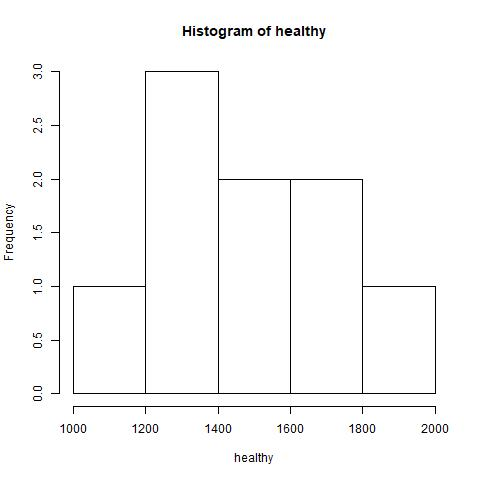
\includegraphics[height=6cm,width=7cm]{healthy.jpg}
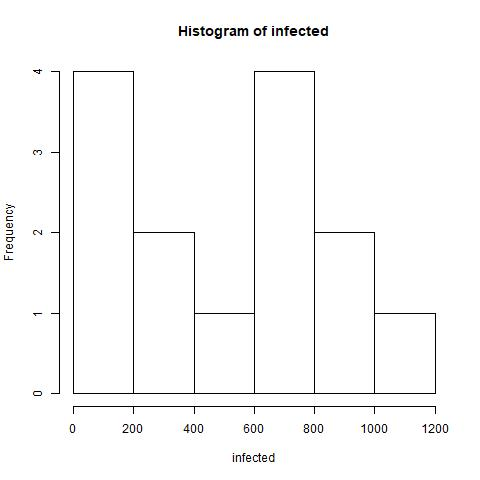
\includegraphics[height=6cm,width=7cm]{infected.jpg}

Difficulties:
\subitem Small sample size:
\subitem How to distinguish between bell-shaped and mound-shaped, but non-normal distribution?

A quantile-quantile (QQ) plot is more reliable tool to assess normality. 
\newline
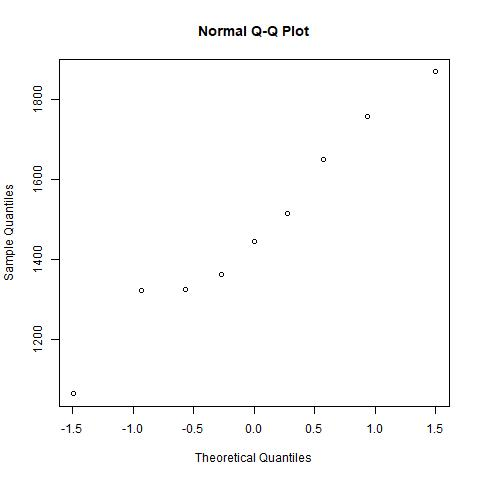
\includegraphics[height=6cm,width=7cm]{healthyqq.jpg}
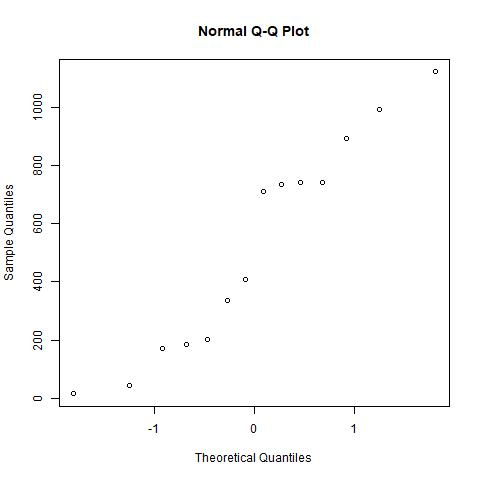
\includegraphics[height=6cm,width=7cm]{infectedqq.jpg}
\item Assessing equal variance
\subitem Box plot
\newline
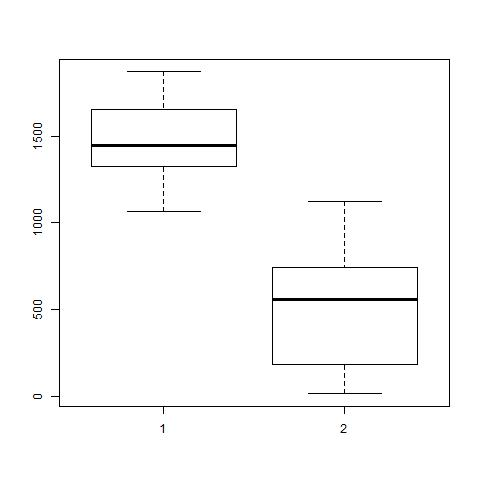
\includegraphics[height=6cm,width=7cm]{box.jpg}
\subitem Levene’s test
By using R, we get the p-value of Levene's test 0.1112, thus ,we cannot reject the null hypothesis under 5\% significance level.
\end{enumerate}
\subparagraph{f)}~{}

Since the two sample variances are obviously different, we perform a Welch’s T test and construct the corresponding 95\% confidence interval for the difference of the mean stem volume of 2-year-old seedlings between the two groups.

We use $t$ statistics \[T=\frac{(\mu_1-\mu_2)-0}{\sqrt{\frac{S_1^2}{n_1}+\frac{S_2^2}{n_2})}}\]
a 95\% confidence interval for the difference of the mean stem volume of 2-year-old seedlings between the two groups is\[(691.1719 , 1227.1138)\]
\subparagraph{g)}~{}

Goal: $H_0 : \mu_1 = \mu_2$ $H_1 : \mu_1 \neq \mu_2$

Re-arrange the data to give the data either healthy or infected and calculate the mean difference which is  930.6

Repeat 10,000 times, count the number of times that the sample mean difference is as large as or larger than the observed sample mean difference  930.6, and compute a p-value as \[2 \times \frac{0}{10000} = 0\]

Conclusion: There is strong evidence against the $H_0$ that t mean stem volumn is the same for the two bud types. Reject the $H_0$ at the α = 0.05 level. 
\subparagraph{h)}
Since the two samples are independent, we choose Wilcoxon test.

Our goal is to test
$H_0$ : The two populations have the same distribution, 

$H_a$ : The two populations have the same shape but different locations.

First, merge the two samples into one combined sample. 

Then, Sort the observations in the combined sample in ascending order and assign each observation a rank. 

Add the ranks corresponding to observations from the first treatment group. Observed rank sum is r1 = 170

 Using R1 as a test statistic and based on the observed r1, conduct a randomization or approximate Z test. From R, p-value = 0
\subparagraph{i)}~{}
\newline
(d) p-value = 6.446e-07 reject the null hypothesis\\
(f) p-value = 2.487e−07  reject the null hypothesis\\
(g) p-value = 0 reject the null hypothesis\\
(h) p-value = 0 reject the null hypothesis
\subparagraph{j)}~{}
we set d=0.8, results for minimum size of $n_1$ and $n_2$ are listed below:
\begin{table}[]
\begin{tabular}{lllllllllllllll}
$n_1$ & 13  & 14  & 15 & 16 & 17 & 18 & 19 & 20 & 21 & 22 & 23 & 24 & 25 & 26 \\
$n_2$ & 250 & 113 & 77 & 60 & 50 & 43 & 39 & 35 & 33 & 31 & 29 & 28 & 27 & 26
\end{tabular}
\end{table}
To make the t test be more robust, the sizes of $n_1$ and $n_2$ should be as same as possible. 
\paragraph{Problem5}
\subparagraph{a)}~{}
\newline
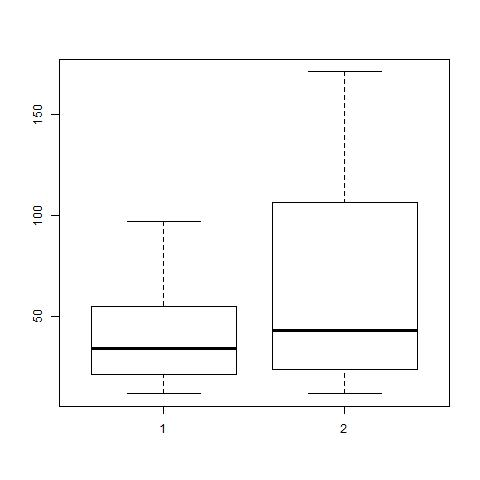
\includegraphics[height=6cm,width=7cm]{5a.jpg}

median(biological)34.5;
median(chemistry)43

mean(biological)41.375;
mean(chemistry)66.25

sd(biological)28.47524;
sd(chemistry)55.91767

Tentative Conclusions: The average of biological control is smaller than chemical control. Chemical control has larger range, which reflects as a larger standard deviation.
\subparagraph{b)}~{}

Hypothesis:\[H_0:\mu_1\ = \mu_2\] \[H_a:\mu_1 \neq \mu_2\]

Two Sample t-test

data:  biological and chemistry

t = -1.1212, df = 14, p-value = 0.2811

alternative hypothesis: true difference in means is not equal to 0

95 percent confidence interval:

 -72.45849  22.70849

sample estimates:

mean of x mean of y 

   41.375    66.250 

Interpretation: under a significance level of 5\%, we cannot reject the null hypothesis.
\subparagraph{c)}~{}

95 percent confidence interval:

 (-72.45849  , 22.70849)
\subparagraph{d)}~{}
\begin{enumerate}
\item Assessing independence
\subitem Consider how the data were collected; that is, the study or experimental design.
\subitem Paired two sample versus unpaired two sample studies.
\subitem The notion of independent observations is closely related to the idea of an i.i.d. sample.
\subitem Not always obvious, as the answer depends on the kinds of scientific questions of interest and the corresponding populations under study.
\item Assessing normality
\newline
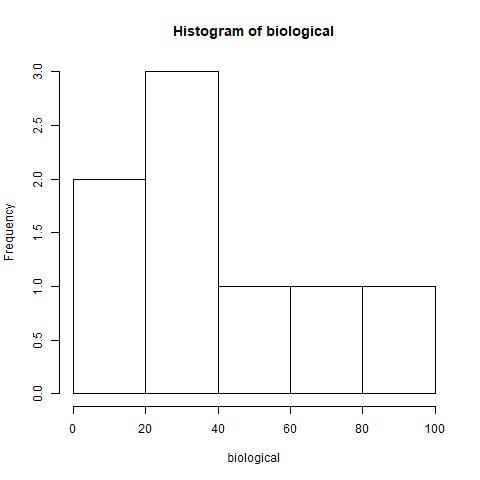
\includegraphics[height=6cm,width=7cm]{biological.jpg}
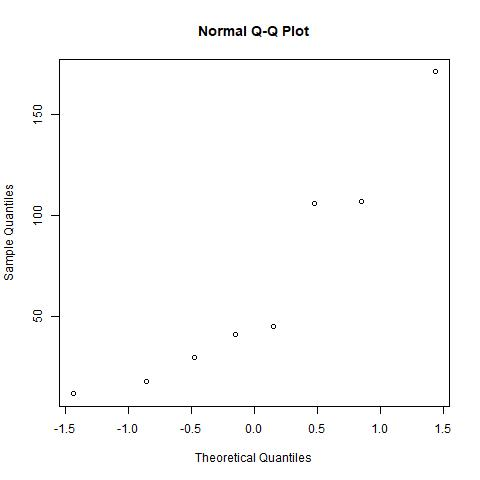
\includegraphics[height=6cm,width=7cm]{chemistry.jpg}

Difficulties:
\subitem Small sample size:
\subitem How to distinguish between bell-shaped and mound-shaped, but non-normal distribution?

A quantile-quantile (QQ) plot is more reliable tool to assess normality. 
\newline
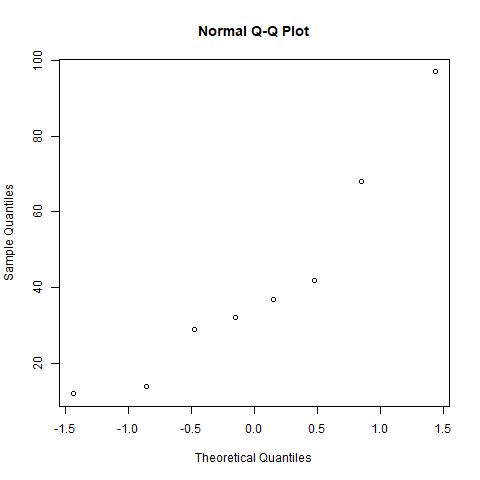
\includegraphics[height=6cm,width=7cm]{biologicalqq.jpg}
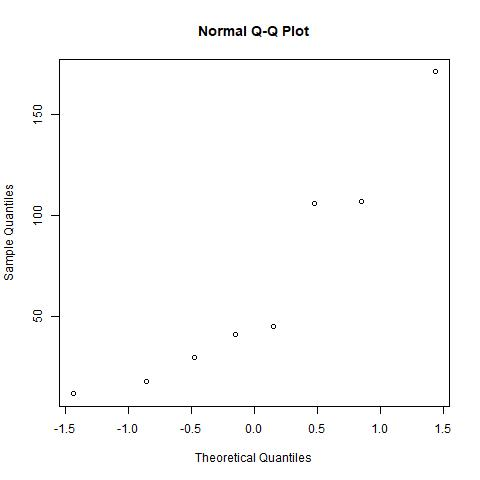
\includegraphics[height=6cm,width=7cm]{chemistryqq.jpg}
\end{enumerate}
\subparagraph{e)}~{}

Welch Two Sample t-test

data:  biological and chemistry

t = -1.1212, df = 10.402, p-value = 0.2874

alternative hypothesis: true difference in means is not equal to 0

95 percent confidence interval:

 -74.05015  24.30015

sample estimates:

mean of x mean of y 

   41.375    66.250 

Interpretation: under a significance level of 5\%, we cannot reject the null hypothesis.
\subparagraph{f)}~{}

Goal: $H_0 : \mu_1 = \mu_2$ $H_1 : \mu_1 \neq \mu_2$

Re-arrange the data to give the data either healthy or infected and calculate the mean difference which is  −24.875.

Repeat 10,000 times, count the number of times that the sample mean difference is as large as or larger than the observed sample mean difference −24.875, and compute a p-value as $p=0.29$

Conclusion: There is no strong evidence against the $H_0$. Accept the $H_0$ at the α = 0.05 level. 
\subparagraph{g)}
For the given samples ae paired, we select Wilcoxon Signed Rank Test 

First, take the sample of differences and compute their absolute values. 

Then, sort the observations in the sample of absolute differences in ascending order and assign each observation a rank. 

 Add the ranks corresponding to the positive values in the original data set and this is the observed test statistic.

Perform a permutation test on this sum of the positive ranks.

Perform a randomization test on this sum of the positive ranks. Repeat 10,000 times, count the number of times that the rank of random sample is as large as or smaller than the observed sample rank 2, and compute a p-value as $p=0.02$

In this case we have to reject the null hypothesis under 5\% significance level.
\subparagraph{h)}~{}
\newline
(b) p-value = 0.2811, we accept the null hypothesis\\
(e) p-value = 0.2874, we accept the null hypothesis\\
(g) p-value=0.02, we reject the null hypothesis
\newpage
\paragraph{Problem6}
\csvautotabular{PM1.csv}

The data above is collected from Tiantan, Beijing in PM 2.5 in 3/1/2013 and 9/1/2013
What we want to do is to test wheather in different seasons the mean density of PM2.5 is the same or not.

To fulfil the goal, we firstly need to guess, and that is what we called $Hypothesis$ in statistics.

And we therefore have two guesses: YES and NO. In statistical terminology, that is \[H_0 : \mu_1 = \mu_2  H_1 : \mu_1 \neq \mu_2\]

Then we need to confirm which one is correct and that is called $testing$ statistically. In this case we will use t test to help us in how much dgree we should reject the equation and usually the dgree is 95\%
And of course we will use R to help us calculate, and the result shows as below:\[t = -13.399,  p-value = 5.013e-13\]
These two statistical values tell us that we should reject the null hypothesis$H_0$  under 5\% of making mistakes.

So, what is the real mean difference between two sample? Since they are all random pheononmena, we cannnot be 100\% sure to say the difference is at a certain point. However, we can find an interval that contains the difference mean. A Confidence Interval(CI) is used to describe such thing. In the case above, the CI is \[(-42.34590 , -31.07077)\]
Now, we finish the hypothesis and testing, also found a reasonable internal to the difference mean.

what if we what to know more about the distribution of PM2.5? Suppose we have adequate data from the history which are randomly collected from a certain distribution with known expection $\mu$ and variance $\sigma^2$, we then calculate \[\frac{S_n-\mu}{\frac{\sigma}{sqrt{n}}}\] 
and the new variable goes to be normally distributed, when n goes to infinity.
\newpage
\appendixpage


the R code used in homework is listed here

2
set.seed(1)

n=10

x=matrix(nrow = n,ncol = 100)

mu=vector(length = 100)

v=vector(length=100)

for (i in 1:100) {

  x[,i]=rnorm(n,mean = 2,sd=2)

  mu[i]=mean(x[,i])

  v[i]=var(x[,i])

}

jpeg("2amean.jpg")

hist(mu)

dev.off()

jpeg("2avar.jpg")

hist(v)

dev.off()

(b),(c) just change n into 40 and 160 respectively

(e)set.seed(1)

n=10

S=10

mu=vector()

v=vector()

x=replicate(100,rbinom(n,S,0.2))

for (i in 1:100) {

mu[i]=mean(x[,i])

v[i]=var(x[,i])

}

jpeg("2emean.jpg")

hist(mu)

dev.off()

jpeg("2evar.jpg")

hist(v)

dev.off()

x=read.csv("Spanish.csv")

y=x[,3]-x[,2]

jpeg("3b.jpg")

plot(y,type = "b")

dev.off

(c)t.test(x[,3],x[,2])

(d)t.test(x[,3],x[,2],conf.level = 0.90)

4)
(a)healthy=c(1870,1324,1446,1325,1759,1652,1364,1515,1065)

infected=c(1121,408,184,16,741,170,991,711,734,202,893,742,335,444)

jpeg("4a.jpg")

plot(healthy,col="red",ylim = c(0,2000))

points(infected,col="blue")

dev.off()

(6)x=read.csv("PM1.csv")

y=x[,2]

z=x[,3]

t.test(y,z)
\end{document}